\documentclass{article}
\usepackage[a4paper, total={6in, 8in}]{geometry}
\usepackage{graphicx, amssymb}

\title{Tecnología Digital VI - Guía de Ejercicios 3}
\author{Juan Ignacio Elosegui}
\date{Noviembre 2025}

\begin{document}
    \maketitle
    \section*{Ejercicio 1}
        \subsection*{Inciso 1}
            \textbf{Falso.} Un perceptrón simple puede representar solamente funciones linealmente separables. Se puede notar por la función que lo define: \(y = \phi(\mathbf{w} \cdot \mathbf{x} + b)\). \\
            Siendo \(\mathbf{x} = [x_{1}, x_{2}, \ldots, x_{n}]\) las entradas, que pueden ser los features. Los pesos \(\mathbf{w} = [w_{1}, w_{2}, \ldots, w_{n}]\) denotan qué tan importante es cada feature. \(b\) es un escalar que funciona como sesgo único (en el caso de un perceptrón simple, ya que tiene una sola salida), pero puede ser un vector de sesgos si tiene varias salidas.
        \subsection*{Inciso 2}
           \textbf{Falso.} Habla de aproximación, no representación directamente. Además, sólo funciona para funciones continuas y solamente si es que el perceptrón tiene activaciones no lineales y suficientes neuronas. Se tienen que dar sí o sí estas cosas para que sea verdadero el enunciado.
        \subsection*{Inciso 3}
            \textbf{Falso.} Por el mismo motivo de arriba, se pueden representar si 1) la función es continua y 2) si el perceptrón tiene las suficientes neuronas.
        \subsection*{Inciso 4}
            \textbf{Falso.} Por el mismo motivo.
        \subsection*{Inciso 5}
            \textbf{Verdadero.} Sí se puede. Una imagen, digamos de dimensión 28 pixeles de alto y ancho, se puede aplanar en un vector de 784 componentes: \(\mathbf{x} \in \mathbb{R}^{784}\). \\
            Este vector se puede pasar por una red neuronal \textit{fully-connected} de la siguiente manera: \(a^{(i)} = \phi\left(\mathbf{W}^{(i)}\mathbf{x} + \mathbf{b}^{(i)}\right)\), donde:
            \begin{itemize}
                \item \(\mathbf{W}^{(i)}\) es la matriz de pesos,
                \item \(\mathbf{x}\) es el vector de 784 entradas,
                \item \(a^{(i)}\) es el vector de activaciones de la capa $i$.
            \end{itemize}
    \section*{Ejercicio 2.1}
        \subsection*{Inciso (a)}
            Tiene 5 unidades de entrada. Son las que están más a la izquierda de la red, en la capa de input.
        \subsection*{Inciso (b)}
            Tiene 3 unidades ocultas. Son las que están en la capa oculta.
        \subsection*{Inciso (c)}
            Tiene una única unidad de salida, es la que está en la capa de output.
        \subsection*{Inciso (d)}
            Cada unidad recibe todas las salidas de la capa anterior como entrada. Cada unidad oculta tiene 5 pesos, y la neurona de salida tiene 3 pesos. Entonces, hay \(5 \cdot 3 + 3 \cdot 1 = 18\) parámetros $w$.
        \subsection*{Inciso (e)}
            Cada unidad de la capa oculta y de salida tiene su propio sesgo. Por lo tanto, hay $3+1 = 9$ sesgos.
        \subsection*{Inciso (f)}
            La salida de la red se obtiene aplicando las transformaciones lineales y las funciones de activación capa por capa. \\
            \\
            \noindent Primera capa oculta:
            \[
                \mathbf{z}^{(1)} = W^{(1)} \mathbf{x} + \mathbf{b}^{(1)},
                \qquad
                \mathbf{a}^{(1)} = \phi\!\left( \mathbf{z}^{(1)} \right),
            \]
            donde
            \[
                W^{(1)} \in \mathbb{R}^{3 \times 5}, \qquad
                \mathbf{x} \in \mathbb{R}^{5}, \qquad
                \mathbf{b}^{(1)} \in \mathbb{R}^{3}, \qquad
                \mathbf{a}^{(1)} \in \mathbb{R}^{3}.
            \]
            \noindent Capa de salida:
            \[
                z^{(2)} = W^{(2)} \mathbf{a}^{(1)} + b^{(2)},
                \qquad
                a^{(2)} = \phi\!\left( z^{(2)} \right),
            \]
            donde
            \[
                W^{(2)} \in \mathbb{R}^{1 \times 3}, 
                \qquad
                b^{(2)} \in \mathbb{R}^{1},
                \qquad
                a^{(2)} \in \mathbb{R}^{1}.
            \]
            \noindent En forma compacta:
            \[
                a^{(2)} = 
                \phi\!\Big(
                W^{(2)} \, \phi\!\left( W^{(1)} \mathbf{x} + \mathbf{b}^{(1)} \right)
                + b^{(2)}
                \Big).
            \]
    \section*{Ejercicio 2.2}
        \subsection*{Inciso (a)}
            Tiene 5 unidades de entrada.
        \subsection*{Inciso (b)}
            Tiene \(6 + 7 + 7 + 6 = 26\) unidades ocultas.
        \subsection*{Inciso (c)}
            Tiene 5 unidades de salida.
        \subsection*{Inciso (d)}
            Tiene \((6 \cdot 5)+(7 \cdot 6)+(7 \cdot 7)+(6 \cdot 7)+(5 \cdot 6) = 193\) parámetros $w$.
        \subsection*{Inciso (e)}
            Tiene \(6+7+7+6+5 = 31\) parámetros $b$.
        \subsection*{Inciso (f)}
            \(\ldots\)
    \section*{Ejercicio 3}
        \subsection*{Función AND}
            Vamos a tener dos inputs a la neurona de entrada, porque la función AND y OR se pueden explicar de manera mínima con dos valores lógicos de \(x_{1}, x_{2} = \{0, 1\}\). Va a tener una sola salida, que será \(\{0, 1\}\), siendo falso o verdadero, respectivamente. \\
            \\
            Se pasan los tres parámetros: $x_{1} \cdot w_{1}$, $x_{2} \cdot w_{2}$ y $b$. En la neurona se suman los parámetros. En la salida, se aplica una función de activación para generar el output $y$.
            \begin{center}
                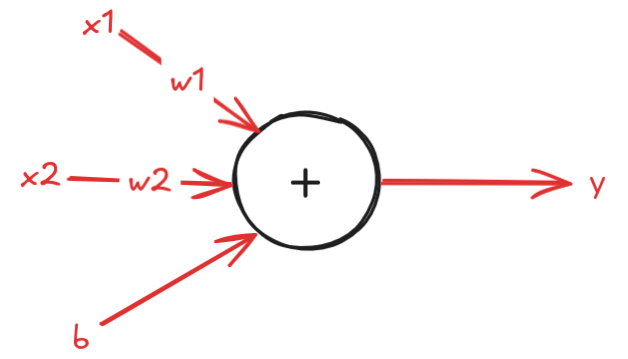
\includegraphics[width=0.5\linewidth]{figs-3/ej3a.png}
            \end{center}
    \section*{Ejercicio 4}
        Ver \texttt{ej4.py}.
    \section*{Ejercicio 5}
       \noindent Los tres (perceptrón, regresión logística y SVM) construyen un hiperplano lineal para separar las clases y usan el mismo tipo de combinación lineal $\mathbf{w} \cdot \mathbf{x} + b$. Pero se diferencian en cómo entrenan, qué función de \textit{loss} usan y qué tipo de salida generan. \\
       \\
       El perceptrón no usa probabilidades, ajusta pesos solo cuando se equivoca y minimiza el error contando cuántas veces se equivocó. \\
       La regresión lineal aplica la función sigmoide para usar una salida probabilística y busca minimizar la log-loss. \\
       SVM busca maximizar el margen, usa la hinge loss y no usa probabilidades.

\end{document}
